\documentclass[12pt]{article}
\usepackage{amsmath}
\usepackage{tikz}
\begin{document}
\title{Computer Science 180, Homework 7}
\date{March 8th, 2018}
\author{Michael Wu\\UID: 404751542}
\maketitle

\section*{Chapter 7, Problem 11}

\begin{center}
        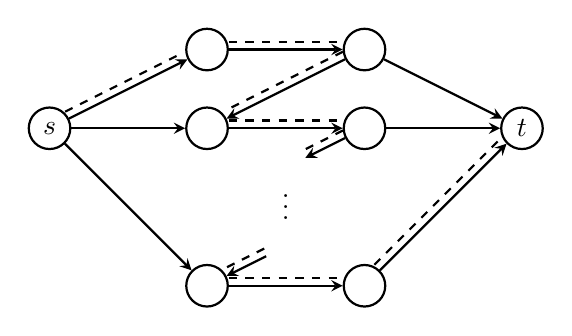
\begin{tikzpicture}
                \begin{scope}[auto, every node/.style={thick, draw,circle,minimum size=1.5em,inner sep=1}, every path/.style={thick, ->, >=stealth}]
                        \node (S) at (0,0) {\(s\)};
                        \node (T) at (6,0) {\(t\)};
                        \node (A) at (2,1) {};
                        \node (B) at (2,0) {};
                        \node (C) at (2,-2) {};
                        \node (D) at (4,1) {};
                        \node (E) at (4,0) {};
                        \node (F) at (4,-2) {};
                        \node [draw=none] (G) at (3,-0.9) {\vdots};
                        \node [draw=none] (H) at (3,-0.5) {};
                        \node [draw=none] (I) at (3,-1.5) {};

                        \path (S) edge (A);
                        \path (S) edge (B);
                        \path (S) edge (C);
                        \path (D) edge (T);
                        \path (E) edge (T);
                        \path (F) edge (T);
                        \path (A) edge (D);
                        \path (B) edge (E);
                        \path (C) edge (F);
                        \path (D) edge (B);
                        \path (E) edge (H);
                        \path (I) edge (C);

               \end{scope}
               \path[thick,dashed,transform canvas={xshift=-0.05cm, yshift=0.0866cm}] (S) edge (A);
               \path[thick,dashed,transform canvas={yshift=0.1cm}] (A) edge (D);
               \path[thick,dashed,transform canvas={xshift=-0.0259cm, yshift=0.0966cm}] (D) edge (B);
               \path[thick,dashed,transform canvas={yshift=0.1cm}] (B) edge (E);
               \path[thick,dashed,transform canvas={xshift=-0.0259cm, yshift=0.0966cm}] (E) edge (H);
               \path[thick,dashed,transform canvas={xshift=-0.0259cm, yshift=0.0966cm}] (I) edge (C);
               \path[thick,dashed,transform canvas={yshift=0.1cm}] (C) edge (F);
               \path[thick,dashed,transform canvas={xshift=-0.0707cm, yshift=0.0707cm}] (F) edge (T);
        \end{tikzpicture}
\end{center}

This statement is false. Consider the graph shown above, where each edge has a capacity of \(1\). There is an arbitrary amount
of rows \(r\) that form paths from the source \(s\) to the sink \(t\), indicated by the vertical dots. Then if the Forward-Edge-Only Algorithm
chooses the path given by the dotted lines, it will terminate with a flow value of \(v(f^\prime)=1\). But
the maximum flow value is \(v(f)=r\), which occurs when every outgoing edge from \(s\) is used. Thus for any constant \(b>1\), we can
create a graph such that the Forward-Edge-Only Algorithm is not guaranteed to find a flow value of at least \(\frac{1}{b}\) times the maximum flow value.
We do this by having \(r>b\) in the graph shown above, then there exists a flow \(f^\prime\) that the Forward-Edge-Only Algorithm can find in this graph where
\[v(f^\prime)=\frac{1}{r}v(f)\]
Thus \(v(f^\prime)\) is \(\frac{1}{r}\) times the maximum flow value, less than \(\frac{1}{b}\) times the maximum flow value.

\pagebreak

\section*{Chapter 7, Problem 14}

\pagebreak

\section*{Chapter 7, Problem 17}

\pagebreak

\section*{Chapter 7, Problem 29}

\end{document}